\begin{lstlisting}
//funcion para comprobar si un vector esta ordenado o no
bool compruebaOrdenado(std::vector<int> v)
{
    for(int i = 0; i < v.size()-1; i++)
    {
        if(v[i] > v[i+1])
            return false;
    }
    return true;
}

int main()
{
    std::vector<int> v;
    std::cout << "[Ordenacion rapida] Para un vector de 5 elementos, 120 combinaciones posibles" << std::endl; 
    for(int i = 0; i < 5; i++)
        v.push_back(i);
    int ordenadas = 0;
    do{
        std::vector<int> aux = v;
        ordenacion_rapida(aux, 0, aux.size());
        if(compruebaOrdenado(aux))
            ordenadas++;
    }while(std::next_permutation(v.begin(), v.end()));
    std::cout << "Numero de permutaciones ordenadas: " << ordenadas << std::endl; 
}
\end{lstlisting}

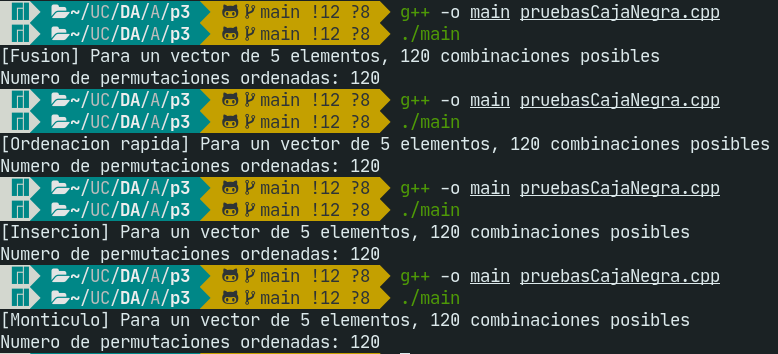
\includegraphics[scale=0.6]{DA.png} 